\section{Traditional security tools}
\label{sec:traditionalsecurity}

For a long time, security has been considered a part of software testing~\cite{sharma2017}.
Security was addressed in a reactive manner, from the end (right) of the \gls{sdlc}, as shown in Figure~\ref{fig:testing}.
Based on vulnerabilities reported when the application was tested after its initial development was completed or when it was already deployed and in production, developer training was adapted, new coding checks were introduced, and \glspl{security problem} were fixed by revisiting code.

\begin{figure}
    \centering
    %
\begin{tikzpicture}[
    scale=0.75
    ]
    
    % SDLC blocks
    \coordinate(a1) at (10.0, 10.0);
    \coordinate(a2) at (10.3, 10.5);
    \coordinate(a3) at (10.0, 11.0);
    \coordinate(a4) at (12.8, 11.0);
    \coordinate(a5) at (13.1, 10.5);
    \coordinate(a6) at (12.8, 10.0);
    \fill[scw-yellow] (a1) -- (a2) -- (a3) -- (a4) -- (a5) -- (a6) -- cycle;
    \node[black] at (11.5,10.5) {\sffamily Plan};
    
    \coordinate(b1) at (13.0, 10.0);
    \coordinate(b2) at (13.3, 10.5);
    \coordinate(b3) at (13.0, 11.0);
    \coordinate(b4) at (15.8, 11.0);
    \coordinate(b5) at (16.1, 10.5);
    \coordinate(b6) at (15.8, 10.0);
    \fill[scw-yellow] (b1) -- (b2) -- (b3) -- (b4) -- (b5) -- (b6) -- cycle;
    \node[black] at (14.5,10.5) {\sffamily Develop};
    
    \coordinate(c1) at (16.0, 10.0);
    \coordinate(c2) at (16.3, 10.5);
    \coordinate(c3) at (16.0, 11.0);
    \coordinate(c4) at (18.8, 11.0);
    \coordinate(c5) at (19.1, 10.5);
    \coordinate(c6) at (18.8, 10.0);
    \fill[scw-yellow] (c1) -- (c2) -- (c3) -- (c4) -- (c5) -- (c6) -- cycle;
    \node[black] at (17.5,10.5) {\sffamily Build};
    
    \coordinate(d1) at (19.0, 10.0);
    \coordinate(d2) at (19.3, 10.5);
    \coordinate(d3) at (19.0, 11.0);
    \coordinate(d4) at (21.8, 11.0);
    \coordinate(d5) at (22.1, 10.5);
    \coordinate(d6) at (21.8, 10.0);
    \fill[scw-yellow] (d1) -- (d2) -- (d3) -- (d4) -- (d5) -- (d6) -- cycle;
    \node[black] at (20.5,10.5) {\sffamily Test};
    
    \coordinate(e1) at (22.0, 10.0);
    \coordinate(e2) at (22.3, 10.5);
    \coordinate(e3) at (22.0, 11.0);
    \coordinate(e4) at (24.8, 11.0);
    \coordinate(e5) at (25.1, 10.5);
    \coordinate(e6) at (24.8, 10.0);
    \fill[scw-yellow] (e1) -- (e2) -- (e3) -- (e4) -- (e5) -- (e6) -- cycle;
    \node[black] at (23.5,10.5) {\sffamily Release};
    
    % arrows -- last to first
    % 5th arrow
        %triangle
    \coordinate(i1) at (24.3, 7.2); 
    \coordinate(i2) at (24.1, 7.0); 
    \coordinate(i3) at (24.3, 6.8); 
    
    \coordinate(i4) at (24.3, 6.9); 
    \coordinate(i5) at (24.8, 6.9); 
        % top
    \coordinate(i6) at (24.8, 9.9); 
    \coordinate(i7) at (24.6, 9.9); 
    
    \coordinate(i8) at (24.6, 7.1); 
    \coordinate(i9) at (24.3, 7.1); 
    
    \node[scw-orange,left] at (24.6,9.2) {\footnotesize Breaches};
    \fill[scw-orange] (i1) -- (i2) -- (i3) -- (i4) -- (i5) -- (i6) -- (i7) -- (i8) -- (i9) -- cycle;
    
    % horizontal
    \coordinate(i10) at (24.15, 7.1); 
    \coordinate(i20) at (24.05, 7.0); 
    \coordinate(i30) at (24.15, 6.9); 
    \coordinate(i40) at (21.85, 6.9); 
    \coordinate(i50) at (21.85, 7.1); 
    \fill[scw-orange] (i10) -- (i20) -- (i30) -- (i40) -- (i50) -- cycle;
    
    
    % 4th arrow
        %triangle
    \coordinate(j1) at (21.3, 7.2); 
    \coordinate(j2) at (21.1, 7.0); 
    \coordinate(j3) at (21.3, 6.8); 
    
    \coordinate(j4) at (21.3, 6.9); 
    \coordinate(j5) at (21.8, 6.9); 
        % top
    \coordinate(j6) at (21.8, 9.9); 
    \coordinate(j7) at (21.6, 9.9); 
    
    \coordinate(j8) at (21.6, 7.1); 
    \coordinate(j9) at (21.3, 7.1); 
    
    \fill[scw-orange] (j1) -- (j2) -- (j3) -- (j4) -- (j5) -- (j6) -- (j7) -- (j8) -- (j9) -- cycle;
    % horizontal
    \node[scw-orange, left] at (21.6,9.2) {\footnotesize Code};
    \node[scw-orange, left] at (21.6,8.7) {\footnotesize analysis};
    \node[scw-orange, left] at (21.6,8) {\footnotesize Penetration};
    \node[scw-orange, left] at (21.6,7.5) {\footnotesize testing};
    
    % horizontal and back up
        %arrow ending top right
    \coordinate(i10) at (21.15, 7.1); 
    \coordinate(i20) at (21.05, 7.0); 
    \coordinate(i30) at (21.15, 6.9); 
    
    \coordinate(i40) at (13.4, 6.9); 
    \coordinate(i50) at (13.4, 9.7); 
        % top   
    \coordinate(i60) at (13.3, 9.7); 
    \coordinate(i70) at (13.5, 9.9); 
    \coordinate(i80) at (13.7, 9.7); 
    
    \coordinate(i90) at (13.6, 9.7); 
    \coordinate(i100) at (13.6, 7.1); 
    \fill[scw-orange] (i10) -- (i20) -- (i30) -- (i40) -- (i50) -- (i60) -- (i70) -- (i80) -- (i90) -- (i100) -- cycle ;
    
    \node[scw-orange, left] at (13.4,9.2) {\footnotesize Fix};
    
    
    
    
    
\end{tikzpicture}
    \includegraphics[page=16]{03-education/figures/tikzfigures.pdf}
  \caption[Security as part of software testing]{Historically, security was considered a part of software testing and addressed from the end (right) of the \gls{sdlc}.}
  \label{fig:testing} 
\end{figure}

Experience has shown, however, that security should not be an afterthought of software development but that it should be addressed earlier in the development. This is not only to minimize costs~\cite{damm2006faults,briand2000comprehensive,baca2008evaluating,layman2007toward}. Shorter feedback loops also result in better learning performance~\cite{syed2015black,whitney2018embedding}. As a result a \emph{shift left} movement is ongoing to try to identify possible \glspl{security problem} as early as possible in the \gls{sdlc}, as illustrated in Figure~\ref{fig:shiftleft}. New project management techniques such as Agile and \gls{devops} encourage fast incremental releases where the developer is also responsible for meeting non-functional requirements such as security.
To support that, testing and deployment of security guidelines needs to be more automated in short feedback loops, thus shifting security left.

\begin{figure}
    \centering
    %
\begin{tikzpicture}[
    scale=0.75
    ]
    
    % SDLC blocks
    \coordinate(a1) at (10.0, 10.0);
    \coordinate(a2) at (10.3, 10.5);
    \coordinate(a3) at (10.0, 11.0);
    \coordinate(a4) at (12.8, 11.0);
    \coordinate(a5) at (13.1, 10.5);
    \coordinate(a6) at (12.8, 10.0);
    \fill[scw-yellow] (a1) -- (a2) -- (a3) -- (a4) -- (a5) -- (a6) -- cycle;
    \node[black] at (11.5,10.5) {\sffamily Plan};
    
    \coordinate(b1) at (13.0, 10.0);
    \coordinate(b2) at (13.3, 10.5);
    \coordinate(b3) at (13.0, 11.0);
    \coordinate(b4) at (15.8, 11.0);
    \coordinate(b5) at (16.1, 10.5);
    \coordinate(b6) at (15.8, 10.0);
    \fill[scw-yellow] (b1) -- (b2) -- (b3) -- (b4) -- (b5) -- (b6) -- cycle;
    \node[black] at (14.5,10.5) {\sffamily Develop};
    
    \coordinate(c1) at (16.0, 10.0);
    \coordinate(c2) at (16.3, 10.5);
    \coordinate(c3) at (16.0, 11.0);
    \coordinate(c4) at (18.8, 11.0);
    \coordinate(c5) at (19.1, 10.5);
    \coordinate(c6) at (18.8, 10.0);
    \fill[scw-yellow] (c1) -- (c2) -- (c3) -- (c4) -- (c5) -- (c6) -- cycle;
    \node[black] at (17.5,10.5) {\sffamily Build};
    
    \coordinate(d1) at (19.0, 10.0);
    \coordinate(d2) at (19.3, 10.5);
    \coordinate(d3) at (19.0, 11.0);
    \coordinate(d4) at (21.8, 11.0);
    \coordinate(d5) at (22.1, 10.5);
    \coordinate(d6) at (21.8, 10.0);
    \fill[scw-yellow] (d1) -- (d2) -- (d3) -- (d4) -- (d5) -- (d6) -- cycle;
    \node[black] at (20.5,10.5) {\sffamily Test};
    
    \coordinate(e1) at (22.0, 10.0);
    \coordinate(e2) at (22.3, 10.5);
    \coordinate(e3) at (22.0, 11.0);
    \coordinate(e4) at (24.8, 11.0);
    \coordinate(e5) at (25.1, 10.5);
    \coordinate(e6) at (24.8, 10.0);
    \fill[scw-yellow] (e1) -- (e2) -- (e3) -- (e4) -- (e5) -- (e6) -- cycle;
    \node[black] at (23.5,10.5) {\sffamily Release};
    
    % arrows -- last to first
    % 5th arrow
        %triangle
    \coordinate(i1) at (24.3, 7.2); 
    \coordinate(i2) at (24.1, 7.0); 
    \coordinate(i3) at (24.3, 6.8); 
    
    \coordinate(i4) at (24.3, 6.9); 
    \coordinate(i5) at (24.8, 6.9); 
        % top
    \coordinate(i6) at (24.8, 9.9); 
    \coordinate(i7) at (24.6, 9.9); 
    
    \coordinate(i8) at (24.6, 7.1); 
    \coordinate(i9) at (24.3, 7.1); 
    
    \node[scw-orange,left] at (24.6,9.2) {\footnotesize Breaches};
    \fill[scw-orange] (i1) -- (i2) -- (i3) -- (i4) -- (i5) -- (i6) -- (i7) -- (i8) -- (i9) -- cycle;
    
    % horizontal
    \coordinate(i10) at (24.15, 7.1); 
    \coordinate(i20) at (24.05, 7.0); 
    \coordinate(i30) at (24.15, 6.9); 
    \coordinate(i40) at (21.85, 6.9); 
    \coordinate(i50) at (21.85, 7.1); 
    \fill[scw-orange] (i10) -- (i20) -- (i30) -- (i40) -- (i50) -- cycle;
    
    
    % 4th arrow
        %triangle
    \coordinate(j1) at (21.3, 7.2); 
    \coordinate(j2) at (21.1, 7.0); 
    \coordinate(j3) at (21.3, 6.8); 
    
    \coordinate(j4) at (21.3, 6.9); 
    \coordinate(j5) at (21.8, 6.9); 
        % top
    \coordinate(j6) at (21.8, 9.9); 
    \coordinate(j7) at (21.6, 9.9); 
    
    \coordinate(j8) at (21.6, 7.1); 
    \coordinate(j9) at (21.3, 7.1); 
    
    \fill[scw-orange] (j1) -- (j2) -- (j3) -- (j4) -- (j5) -- (j6) -- (j7) -- (j8) -- (j9) -- cycle;
    % horizontal
    \coordinate(i10) at (21.15, 7.1); 
    \coordinate(i20) at (21.05, 7.0); 
    \coordinate(i30) at (21.15, 6.9); 
    \coordinate(i40) at (18.85, 6.9); 
    \coordinate(i50) at (18.85, 7.1); 
    \fill[scw-orange] (i10) -- (i20) -- (i30) -- (i40) -- (i50) -- cycle;
    \node[scw-orange, left] at (21.6,9.2) {\footnotesize Code};
    \node[scw-orange, left] at (21.6,8.7) {\footnotesize analysis};
    \node[scw-orange, left] at (21.6,8) {\footnotesize Penetration};
    \node[scw-orange, left] at (21.6,7.5) {\footnotesize testing};
    
    % 3th arrow
        %triangle
    \coordinate(j1) at (18.3, 7.2); 
    \coordinate(j2) at (18.1, 7.0); 
    \coordinate(j3) at (18.3, 6.8); 
    \coordinate(j4) at (18.3, 6.9); 
    \coordinate(j5) at (18.8, 6.9); 
    \coordinate(j6) at (18.8, 9.9); 
    \coordinate(j7) at (18.6, 9.9); 
    \coordinate(j8) at (18.6, 7.1); 
    \coordinate(j9) at (18.3, 7.1); 
    \fill[scw-orange] (j1) -- (j2) -- (j3) -- (j4) -- (j5) -- (j6) -- (j7) -- (j8) -- (j9) -- cycle;
    % horizontal
    \coordinate(i10) at (18.15, 7.1); 
    \coordinate(i20) at (18.05, 7.0); 
    \coordinate(i30) at (18.15, 6.9); 
    \coordinate(i40) at (15.85, 6.9); 
    \coordinate(i50) at (15.85, 7.1); 
    \fill[scw-orange] (i10) -- (i20) -- (i30) -- (i40) -- (i50) -- cycle;
   
    \node[scw-orange, left] at (18.6,9.2) {\footnotesize Code};
    \node[scw-orange, left] at (18.6,8.7) {\footnotesize analysis};
    
    % 3th arrow
        %triangle
    \coordinate(j1) at (15.3, 7.2); 
    \coordinate(j2) at (15.1, 7.0); 
    \coordinate(j3) at (15.3, 6.8); 
    \coordinate(j4) at (15.3, 6.9); 
    \coordinate(j5) at (15.8, 6.9); 
    \coordinate(j6) at (15.8, 9.9); 
    \coordinate(j7) at (15.6, 9.9); 
    \coordinate(j8) at (15.6, 7.1); 
    \coordinate(j9) at (15.3, 7.1); 
    \fill[scw-orange] (j1) -- (j2) -- (j3) -- (j4) -- (j5) -- (j6) -- (j7) -- (j8) -- (j9) -- cycle;
    
    % horizontal and back up
        %arrow ending top right
    \coordinate(i10) at (15.15, 7.1); 
    \coordinate(i20) at (15.05, 7.0); 
    \coordinate(i30) at (15.15, 6.9); 
    
    \coordinate(i40) at (13.4, 6.9); 
    \coordinate(i50) at (13.4, 9.7); 
        % top   
    \coordinate(i60) at (13.3, 9.7); 
    \coordinate(i70) at (13.5, 9.9); 
    \coordinate(i80) at (13.7, 9.7); 
    
    \coordinate(i90) at (13.6, 9.7); 
    \coordinate(i100) at (13.6, 7.1); 
    \fill[scw-orange] (i10) -- (i20) -- (i30) -- (i40) -- (i50) -- (i60) -- (i70) -- (i80) -- (i90) -- (i100) -- cycle ;
    
    \node[scw-orange, left] at (15.6,9.2) {\footnotesize Code};
    \node[scw-orange, left] at (15.6,8.7) {\footnotesize review};
    
    \node[scw-orange, left] at (13.4,9.2) {\footnotesize Fix};
    
\end{tikzpicture}
    \includegraphics[page=15]{03-education/figures/tikzfigures.pdf}
  \caption[Shift left movement]{In the shift left movement, security practices are shifting left in the \gls{sdlc}. This results in shorter feedback loops, but is still using a reactive approach to find problems after they have been introduced.}
  \label{fig:shiftleft} 
\end{figure}

While supporting the shift left, conventional \gls{vulnerability} scanning tools still use a reactive, testing-based approach. Furthermore, in training developers are typically taught how certain mistakes lead to vulnerabilities, and how these can be exploited. Afterwards they are taught how to prevent the presented vulnerabilities. These practices are extended into the development phase, where the focus is still on the (sometimes complex) question of whether or not the code is vulnerable, and only if it is considered to be vulnerable, it becomes a candidate to be fixed. The shift left movement is certainly an improvement, but it is not yet perfect. Many security problems still occur. Companies acknowledge this, as is obvious from the incentives they put in place to minimize the impact of potential breaches, such as bug bounty programs.

Many of the vulnerability scanning tools use complex control flow and data flow analyses to scan for vulnerabilities in the product. They identify, e.g., user input that is not properly validated and passed on to security-critical parts of the application. If it is determined that a malicious input exists that can cause unwanted or unexpected results, these issues are placed into the \gls{bugtracker} for developers to deal with. In order to successfully detect vulnerabilities, the calling context of routines needs to be known in order to perform the necessary global analyses. Because of this, such tools can only be deployed at a later stage in development. It is, in other words, not possible to shift even more to the left with only these tools. During the earlier development stages of a product, it is entirely possible that no user input can reach a buggy routine yet. The classic approach will only flag the routine once the context exists where it can be exploited. This then requires the developers to go back to secure the routine at a later time than when they were originally developing it. 

In short, even in the ongoing shift left movement, the problem is still approached from the right side of the \gls{sdlc}, following the detection of vulnerabilities. The detection is shifted as much to the left as possible but the approach is still reactive, and requires revisiting code (possibly long) after it has been developed. 

\section{Tools for the paved path methodology}
%Paved path: lay out guidelines early
%No focus on vulnerable or not
%Follow path regardless of context
%Protection for future use
In the paved path methodology we try to avoid this reactive approach.
Instead, the goal is to prevent the introduction of \glspl{security problem} as much as possible, as shown in Figure~\ref{fig:pavedpath}.
This is achieved by laying out guidelines early in the process and enforcing them regardless of the calling context of the code. 
In code that does not take user input, and hence is not likely to result in vulnerabilities, the guidelines are still enforced.
It is after all possible that in the future a calling context will be developed that does take user input.
The code may become vulnerable at that point.
Securing this code fragment from the start will protect it for future use and avoids the need to revisit and fix it when such a calling context exists.
This practice is often called ``establishing secure defaults", and it is part of a ``security by design" approach in software engineering\footurl{https://wiki.owasp.org/index.php/Security\_by\_Design_Principles}

\begin{figure}
    \centering
    %
\begin{tikzpicture}[
    scale=0.75
    ]
    
    % SDLC blocks
    \coordinate(a1) at (10.0, 10.0);
    \coordinate(a2) at (10.3, 10.5);
    \coordinate(a3) at (10.0, 11.0);
    \coordinate(a4) at (12.8, 11.0);
    \coordinate(a5) at (13.1, 10.5);
    \coordinate(a6) at (12.8, 10.0);
    \fill[scw-yellow] (a1) -- (a2) -- (a3) -- (a4) -- (a5) -- (a6) -- cycle;
    \node[black] at (11.5,10.5) {\sffamily Plan};
    
    \coordinate(b1) at (13.0, 10.0);
    \coordinate(b2) at (13.3, 10.5);
    \coordinate(b3) at (13.0, 11.0);
    \coordinate(b4) at (15.8, 11.0);
    \coordinate(b5) at (16.1, 10.5);
    \coordinate(b6) at (15.8, 10.0);
    \fill[scw-yellow] (b1) -- (b2) -- (b3) -- (b4) -- (b5) -- (b6) -- cycle;
    \node[black] at (14.5,10.5) {\sffamily Develop};
    
    \coordinate(c1) at (16.0, 10.0);
    \coordinate(c2) at (16.3, 10.5);
    \coordinate(c3) at (16.0, 11.0);
    \coordinate(c4) at (18.8, 11.0);
    \coordinate(c5) at (19.1, 10.5);
    \coordinate(c6) at (18.8, 10.0);
    \fill[scw-yellow] (c1) -- (c2) -- (c3) -- (c4) -- (c5) -- (c6) -- cycle;
    \node[black] at (17.5,10.5) {\sffamily Build};
    
    \coordinate(d1) at (19.0, 10.0);
    \coordinate(d2) at (19.3, 10.5);
    \coordinate(d3) at (19.0, 11.0);
    \coordinate(d4) at (21.8, 11.0);
    \coordinate(d5) at (22.1, 10.5);
    \coordinate(d6) at (21.8, 10.0);
    \fill[scw-yellow] (d1) -- (d2) -- (d3) -- (d4) -- (d5) -- (d6) -- cycle;
    \node[black] at (20.5,10.5) {\sffamily Test};
    
    \coordinate(e1) at (22.0, 10.0);
    \coordinate(e2) at (22.3, 10.5);
    \coordinate(e3) at (22.0, 11.0);
    \coordinate(e4) at (24.8, 11.0);
    \coordinate(e5) at (25.1, 10.5);
    \coordinate(e6) at (24.8, 10.0);
    \fill[scw-yellow] (e1) -- (e2) -- (e3) -- (e4) -- (e5) -- (e6) -- cycle;
    \node[black] at (23.5,10.5) {\sffamily Release};
    
    % arrows -- last to first
    % 5th arrow
        %triangle
    \coordinate(i1) at (24.3, 9.2); 
    \coordinate(i2) at (24.1, 9.0); 
    \coordinate(i3) at (24.3, 8.8); 
    
    \coordinate(i4) at (24.3, 8.9); 
    \coordinate(i5) at (24.8, 8.9); 
        % top
    \coordinate(i6) at (24.8, 9.9); 
    \coordinate(i7) at (24.6, 9.9); 
    
    \coordinate(i8) at (24.6, 9.1); 
    \coordinate(i9) at (24.3, 9.1); 
    
    \fill[scw-orange] (i1) -- (i2) -- (i3) -- (i4) -- (i5) -- (i6) -- (i7) -- (i8) -- (i9) -- cycle;
    
    % horizontal
    \coordinate(i10) at (24.15, 9.1); 
    \coordinate(i20) at (24.05, 9.0); 
    \coordinate(i30) at (24.15, 8.9); 
    \coordinate(i40) at (21.85, 8.9); 
    \coordinate(i50) at (21.85, 9.1); 
    \fill[scw-orange] (i10) -- (i20) -- (i30) -- (i40) -- (i50) -- cycle;
    
    
    % 4th arrow
        %triangle
    \coordinate(j1) at (21.3, 9.2); 
    \coordinate(j2) at (21.1, 9.0); 
    \coordinate(j3) at (21.3, 8.8); 
    
    \coordinate(j4) at (21.3, 8.9); 
    \coordinate(j5) at (21.8, 8.9); 
        % top
    \coordinate(j6) at (21.8, 9.9); 
    \coordinate(j7) at (21.6, 9.9); 
    
    \coordinate(j8) at (21.6, 9.1); 
    \coordinate(j9) at (21.3, 9.1); 
    
    \fill[scw-orange] (j1) -- (j2) -- (j3) -- (j4) -- (j5) -- (j6) -- (j7) -- (j8) -- (j9) -- cycle;
    % horizontal
    \coordinate(i10) at (21.15, 9.1); 
    \coordinate(i20) at (21.05, 9.0); 
    \coordinate(i30) at (21.15, 8.9); 
    \coordinate(i40) at (18.85, 8.9); 
    \coordinate(i50) at (18.85, 9.1); 
    \fill[scw-orange] (i10) -- (i20) -- (i30) -- (i40) -- (i50) -- cycle;
    
    % 3th arrow
        %triangle
    \coordinate(j1) at (18.3, 9.2); 
    \coordinate(j2) at (18.1, 9.0); 
    \coordinate(j3) at (18.3, 8.8); 
    \coordinate(j4) at (18.3, 8.9); 
    \coordinate(j5) at (18.8, 8.9); 
    \coordinate(j6) at (18.8, 9.9); 
    \coordinate(j7) at (18.6, 9.9); 
    \coordinate(j8) at (18.6, 9.1); 
    \coordinate(j9) at (18.3, 9.1); 
    \fill[scw-orange] (j1) -- (j2) -- (j3) -- (j4) -- (j5) -- (j6) -- (j7) -- (j8) -- (j9) -- cycle;
    % horizontal
    \coordinate(i10) at (18.15, 9.1); 
    \coordinate(i20) at (18.05, 9.0); 
    \coordinate(i30) at (18.15, 8.9); 
    \coordinate(i40) at (15.85, 8.9); 
    \coordinate(i50) at (15.85, 9.1); 
    \fill[scw-orange] (i10) -- (i20) -- (i30) -- (i40) -- (i50) -- cycle;
   
    
    % 3th arrow
        %triangle
    \coordinate(j1) at (15.3, 9.2); 
    \coordinate(j2) at (15.1, 9.0); 
    \coordinate(j3) at (15.3, 8.8); 
    \coordinate(j4) at (15.3, 8.9); 
    \coordinate(j5) at (15.8, 8.9); 
    \coordinate(j6) at (15.8, 9.9); 
    \coordinate(j7) at (15.6, 9.9); 
    \coordinate(j8) at (15.6, 9.1); 
    \coordinate(j9) at (15.3, 9.1); 
    \fill[scw-orange] (j1) -- (j2) -- (j3) -- (j4) -- (j5) -- (j6) -- (j7) -- (j8) -- (j9) -- cycle;
    
    % horizontal and back up
        %arrow ending top right
    \coordinate(i10) at (15.15, 9.1); 
    \coordinate(i20) at (15.05, 9.0); 
    \coordinate(i30) at (15.15, 8.9); 
    
    \coordinate(i40) at (13.6, 8.9); 
    \coordinate(i50) at (13.6, 9.7); 
        % top   
    \coordinate(i60) at (13.5, 9.7); 
    \coordinate(i70) at (13.7, 9.9); 
    \coordinate(i80) at (13.9, 9.7); 
    
    \coordinate(i90) at (13.8, 9.7); 
    \coordinate(i100) at (13.8, 9.1); 
    \fill[scw-orange] (i10) -- (i20) -- (i30) -- (i40) -- (i50) -- (i60) -- (i70) -- (i80) -- (i90) -- (i100) -- cycle ;
    
    \node[scw-orange, below] at   (15.3, 9) {\footnotesize Security problems};
    \node[scw-teal, below] at (12.3, 9) {\footnotesize Guidelines};
    
    % preventative arrow
        %arrow point
    \coordinate(p1) at (13, 9.7); 
    \coordinate(p2) at (13.2, 9.9); 
    \coordinate(p3) at (13.4, 9.7); 
    \coordinate(p4) at (13.3, 9.7); 
    \coordinate(p5) at (13.3, 8.9); 
    \coordinate(p6) at (11.3, 8.9); 
    \coordinate(p7) at (11.3, 9.9); 
    \coordinate(p8) at (11.5, 9.9); 
    \coordinate(p9) at (11.5, 9.1); 
    \coordinate(p10) at (13.1, 9.1); 
    \coordinate(p11) at (13.1, 9.7); 
    
    \fill[scw-teal] (p1) -- (p2) -- (p3) -- (p4) -- (p5) -- (p6) -- (p7) -- (p8) -- (p9) -- (p10) -- (p11) -- cycle;
    
\end{tikzpicture}
    \includegraphics[page=14]{03-education/figures/tikzfigures.pdf}
  \caption[Paved path methodology]{The paved path methodology introduces a preventative approach. This is done by creating guidelines that, when adhered to, will help prevent the introduction of security problems.}
  \label{fig:pavedpath} 
\end{figure}

%Achieve the goals set out in the vision through these features:
This fundamentally different approach of enforcing (secure) coding guidelines instead of scanning for vulnerabilities, makes it possible to meet the requirements for tools supporting the paved path methodology, such as Sensei.
Sensei is an \gls{ide} plugin developed by \gls{scw} with the goal of helping developers produce more secure code.
It is currently available for IntelliJ IDEA and Android Studio, it supports Java, Kotlin and \gls{xml}.
Sensei can be used by \gls{devsecops} teams to apply the paved path methodology in their software development process.
As described in Chapter~\ref{ch:vision}, to support the paved path methodology, Sensei needs to be \textit{relevant}, \textit{efficient}, and \textit{usable}.

%Relevant:
%customizable guidelines --> sharing of knowledge
In order to be \textit{relevant} to the developer's work, the paved path methodology prescribes to create API-level guidelines that determine which libraries and even which library calls are to be used in the project.
Custom (wrapper) libraries may need to be developed that are inherently safe so they can be freely used by developers.
To meet this requirement, the guidelines enforced by Sensei need to be easy to customize.
For this purpose Sensei offers a custom editor inside the \gls{ide} which will be discussed in more detail in Chapter~\ref{ch:sensei}.
Easy customization of the guidelines enables security experts and developers to efficiently create and enforce new guidelines as a way to share their knowledge among the rest of the team.

%Efficient:
%local analyses
%quickfixes in the IDE 
%make info available in the IDE
Sensei is designed to be a developer tool in the first place.
It is \textit{efficient} as it improves developer productivity instead of hurting it.
Sensei enforces coding guidelines regardless of context.
Since the context can be ignored, it only needs to perform local code analyses that can be completed in real time, similar to an as-you-type spell checker.
Also similar to a spell checker, Sensei provides an easy way to remediate guideline violations in the form of quick-fixes.
\todo{"These code transformations" refers to the quick-fixes}
These code transformations are an existing \gls{ide} feature that the developer is familiar with.
They are commonly used for marking syntax errors and general coding best practices.
With quick-fixes it is possible to avoid the need for research and even automate the remediation of guideline violations, which greatly improves the productivity of the developer.

Quick-fixes turn the task of fixing insecure code into one where the developer has to \textit{recognize} the correct solution, rather than \textit{recollect}, reducing the cognitive effort and improving \textit{usability}.
Sensei and its quick-fixes are also used by developers for other purposes than security, as will be discussed in the next chapters.
Because the tool resides in the \gls{ide} and reuses existing \gls{ide} features it quickly feels like a simple extension of the existing developer tool kit.